\documentclass{article}
\usepackage[margin=3cm]{geometry}
\usepackage{float}
\usepackage{graphicx}
\usepackage{amsmath}
\usepackage{soul}

\begin{document}

\section{Modelo}

Utilizamos el modelo estándar de red de flujo adaptativo, añadiendole leyes de crecimiento. Cada ducto (vertice entre los nodos $i$ y $j$) posee un largo $l_{ij}$ y
una conductancia $C_{ij}$. La red comienza como un solo ducto (dos nodos conectados) de largo $l_0 + \eta (t)$ y conductancia ideal. 

\st{Cada iteración, una punta (nodo de conectividad 1 diferente del sumidero)es elegida al azar. Luego, ese nodo puede:}
Cada iteración, se calculan las probabilidades de todas las puntas de realizar una de las siguientes acciones:
\begin{itemize}

    \item Crecer ($l_{ij}$ crece de $l_0 + \eta (t)$) con probabilidad $f(C_{ij}) = \frac{1}{2}(1 - e^{-C_{ij}/\bar{C}})$
    \item Bifurcarse (nacen 2 nodos/ductos nuevos) con probabilidad $g(C_{ij}) = f(C_{ij})$
    \item Retraerse ($l_{ij}$ se reduce, si baja de 0 el nodo desaparece) con probabilidad $h(C_{ij}) = e^{-C_{ij}/\bar{C}}$

\end{itemize} 

Se elige entonces la punta y la acción a partir de estas probabilidades.

La red es atravesada por un fluido, introducido por las puntas con flujo $0$ o $2q^{(0)}$ con igual proabilidad.\\
Luego de cada iteración, \st{las conductancias se optimizan} se calculan las conductancias óptimas para minimizar la disipación de energía y mantener un volumen constante (dado por $K$):
$$ C_{ij}^* = \frac{\langle Q_{ij}(t)^2\rangle_T^{2/3} \mathcal{K}}{\left( \sum_{<ij>} \langle Q_{ij}(t)^2\rangle_T^{1/3} l_{ij}\right)^2 l_{ij}} $$

Entonces, la conductancia siguiente es \textbf{POR AHORA, DEBERIA DEPENDER DE $\tau$}:
$$ C_{ij}(t + \Delta t) = \frac{C_{ij}^*(t) - C_{}}{} $$

A cada paso de tiempo ocurre una sola acción. Para estimar el tiempo entre cada evento utilizamos intervalo $\tau$ dado por
el algoritmo de Gillespie: 
$$\tau = \frac{-\ln(r)}{\sum_{ij}f(C_{ij})+g(C_{ij})+h(C_{ij})} = \frac{-\ln(r)}{N}$$
Donde $r\in[0,1]$ es un número aleatorio y $N$ es el número de puntas.

\section{Evolución temporal}

La dinámica de la red posee dos fases bastante claras: 
La primera, la fase de exploración, donde existe un crecimiento rápido del tamaño,
la dinámica está dominada por las bifurcaciones y el crecimiento de los ductos.
Luego, el árbol alcanza un tamaño máximo y comienza a retraerse, teniendo hacia un equilibrio donde
la cantidad de nodos oscila en valores pequeños, pero el largo total se mantiene cerca del máximo: La red se optimiza.

Para las figuras, tomamos como ejemplo un sistema con $K = 100$ y $\bar{C} = 10^{-5}C_0$.

\textbf{AÑADIR GRAFOS}
\newpage
\begin{figure}[h!]
    \centering
    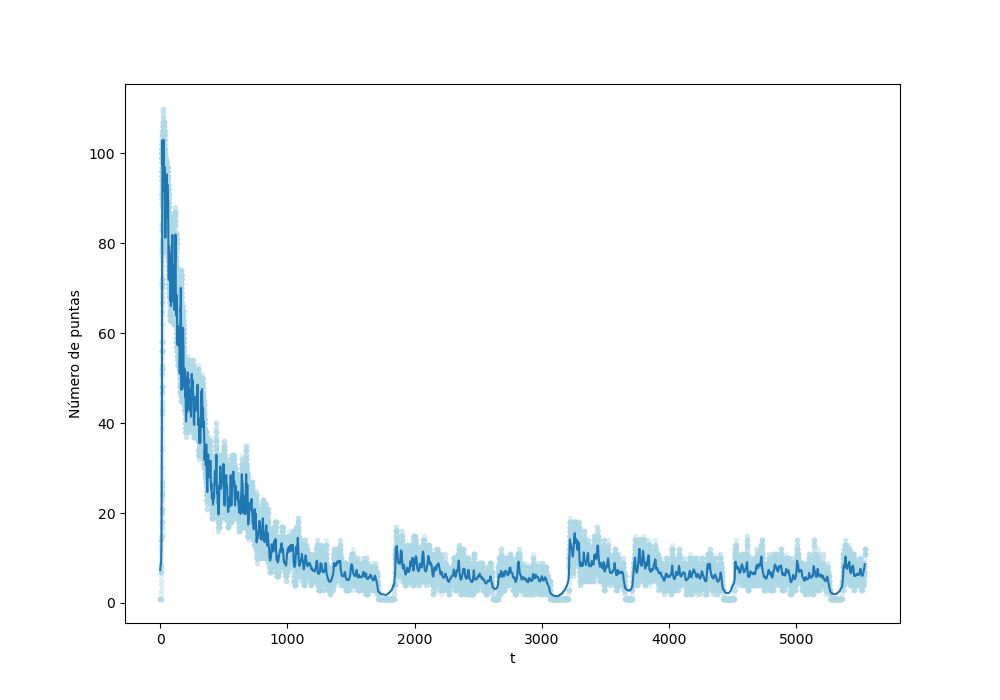
\includegraphics[width=0.7\textwidth]{graficos_inst/N_vs_tiempo.png}
    \caption{Evolución temporal de la cantidad de puntas.}
    \label{fig:evolucion_N}
\end{figure}
La cantidad de bifurcaciones es simplemente el doble.
\begin{figure}[h!]
    \centering
    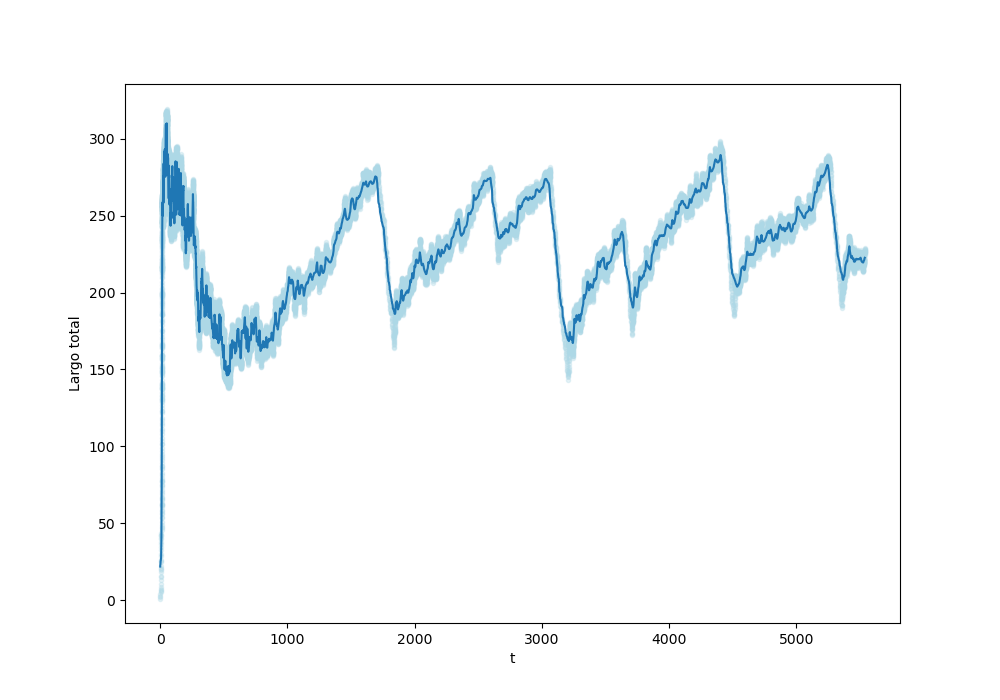
\includegraphics[width=0.7\textwidth]{graficos_inst/largo_vs_tiempo.png}
    \caption{Evolución temporal del largo total del árbol.}
    \label{fig:evolucion_tamano}
\end{figure}

\newpage

La evolución de las probabilidades refleja estas fases, mostrando la dominancia de una u otra acción.

\begin{figure}[h!]
    \centering
    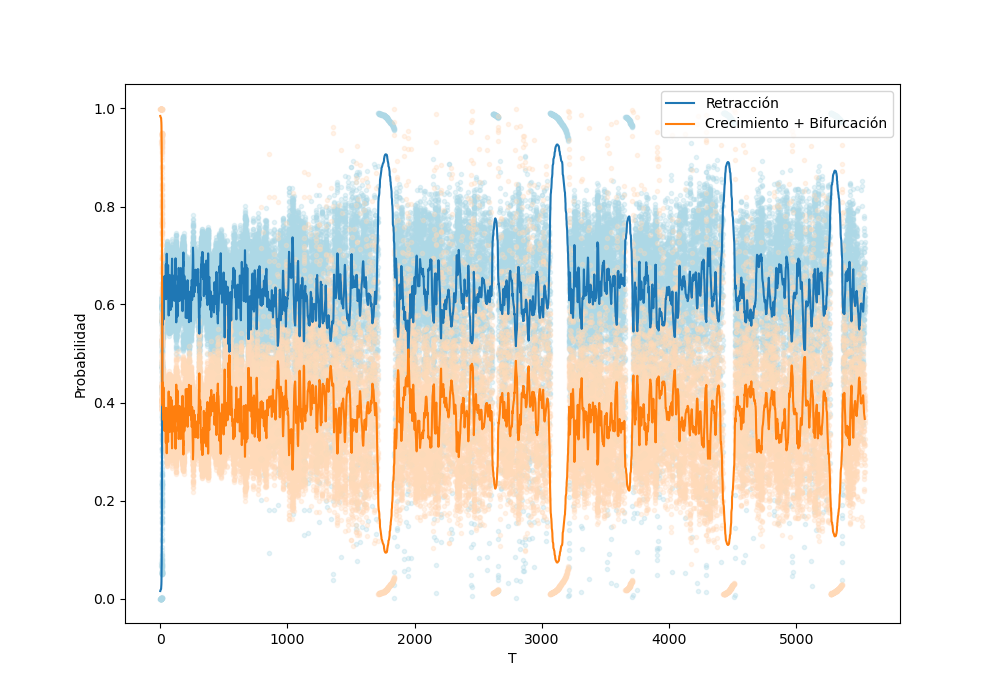
\includegraphics[width=0.8\textwidth]{graficos_inst/probs_vs_tiempo.png}
    \caption{Evolución temporal de las probabilidades promedio.}
    \label{fig:evolucion_probabilidades}
\end{figure}

Finalmente, la conductancia promedio de las puntas converge con el tiempo, a un valor ligeramente inferior?? a la conductancia crítica.

\begin{figure}[h!]
    \centering
    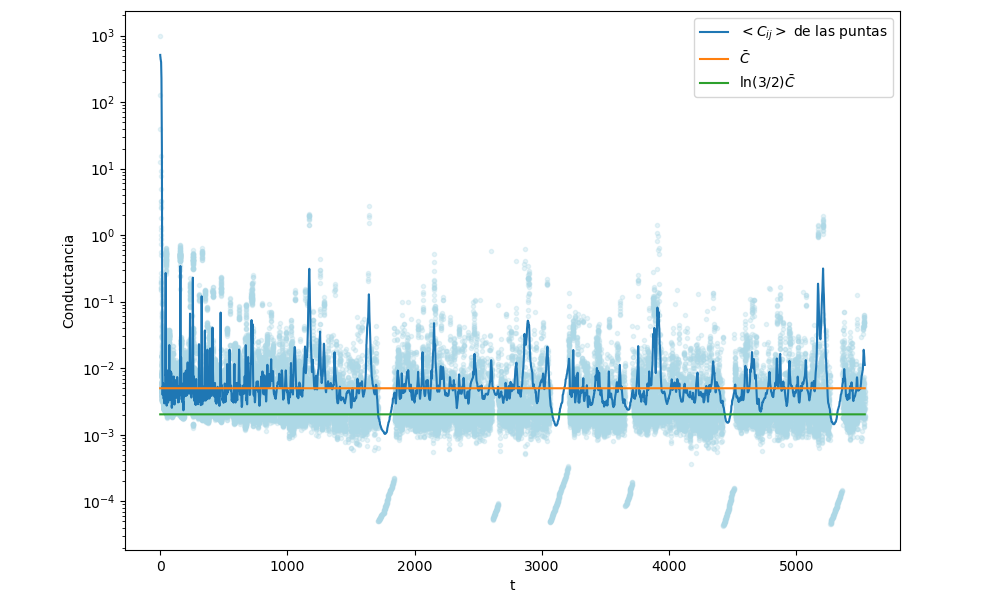
\includegraphics[width=0.65\textwidth]{graficos_inst/Cij_vs_tiempo.png}
    \caption{Evolución temporal de la conductancia.}
    \label{fig:evolucion_conductancia}
\end{figure}
\newpage

Todos los gráficos tienen unos peaks comunes, que corresponden a fuertes retracciones del árbol:
Cuando el primer ducto, o uno de los más antiguos, se vuelve una punta (i.e, \textbf{cuando N es muy pequeño}), su conductancia es muy baja por su largo.
Tiende a retraerse (\textbf{aumenta la probabilidad de retracción}) y lo hace con probabilidad casi 1 hasta alcanzar un C mayor (\textbf{baja la suma de los largos}).
En este punto, se bifurca en dos pequeños ductos con alta conductancia (sube el promedio) y alta probabilidad de crecimiento. \large\textbf{EXPLICAR MEJOR}

\section{Fase de exploración}

Estudiemos la evolución del arbol durante la fase de crecimiento.

\begin{figure}[h!]
    \centering
    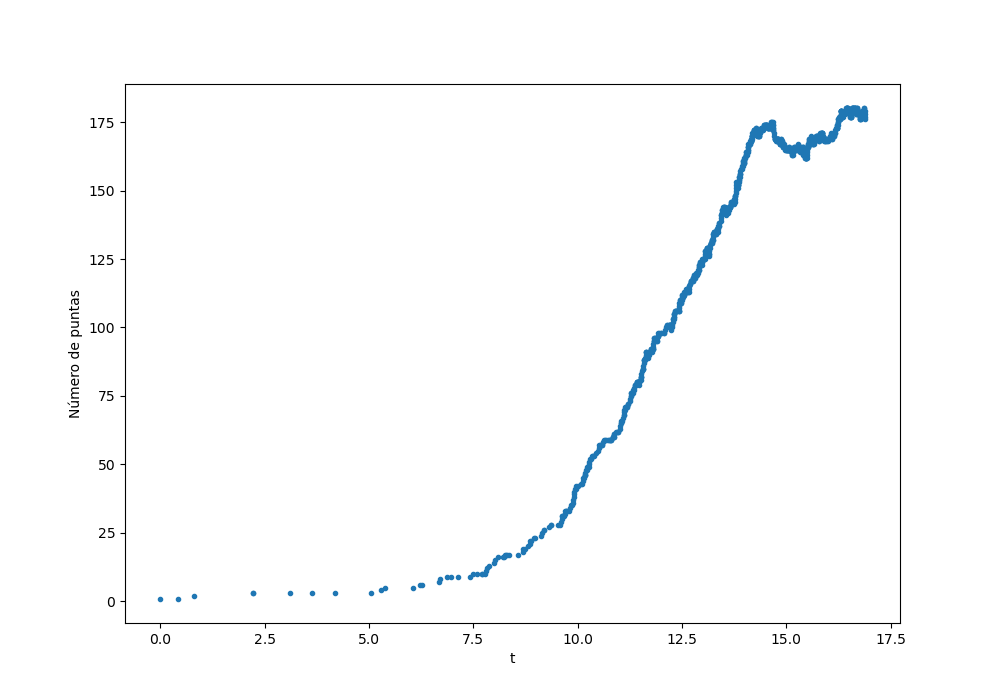
\includegraphics[width=0.65\textwidth]{graficos_inst/N_vs_tiempo_principio.png}
    \caption{Crecimiento de la cantidad de puntas.}
    \label{fig:evolucion_N_principio}
\end{figure}

\begin{figure}[h!]
    \centering
    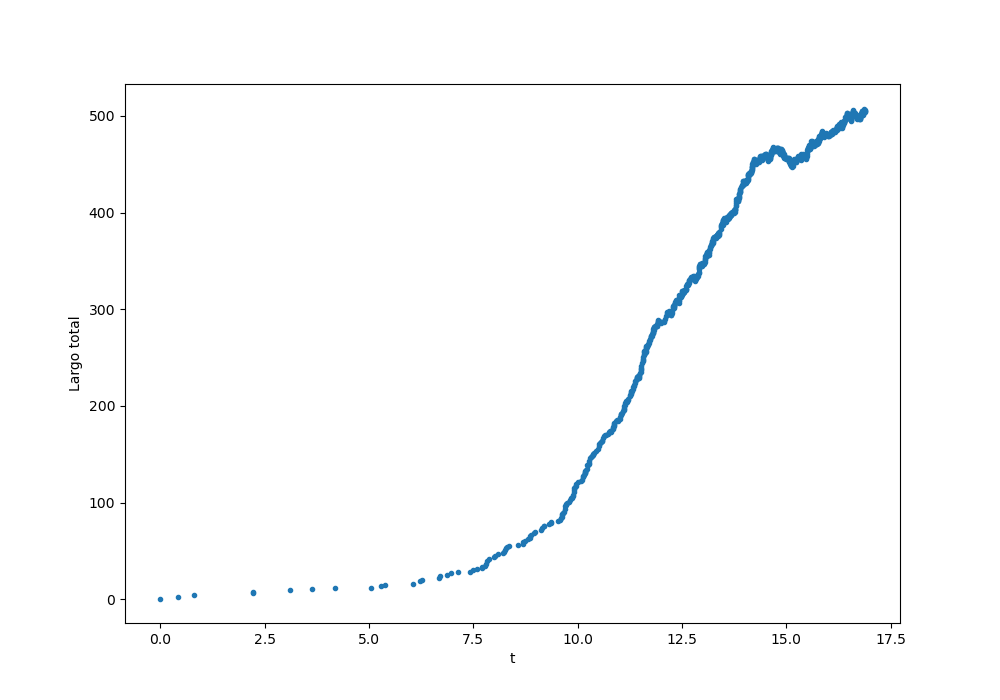
\includegraphics[width=0.65\textwidth]{graficos_inst/largo_vs_tiempo_principio.png}
    \caption{Crecimiento del largo total.}
    \label{fig:evolucion_l_principio}
\end{figure}

Ambos gráficos, en esta fase básicamente proporcionales de factor $2l_0$, muestran un crecimiento exponencial.
En efecto, 

\section{Cambio de fase}

Nos interesamos ahora al cambio de fase. Si vemos más de cerca la evolución del ta

\section{Tamaño máximo \textbf{TODO MALO ACÁ}}

Estudiamos qué determina el tamaño máximo alcanzado por el árbol.

En primer lugar, vemos si $K$ (el volumen del sistema) determina esto. Estudiamos el largo máximo en diferentes simulaciones, variando K y 
fijando las otras variables.

\begin{figure}[h!]
    \centering
    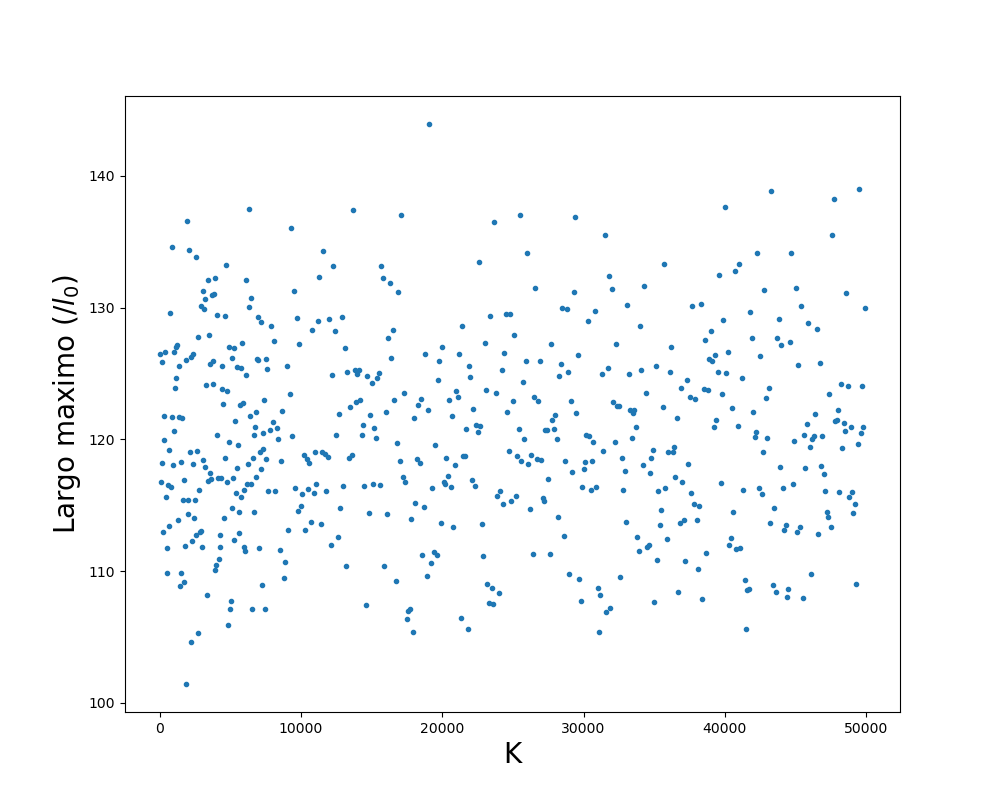
\includegraphics[width=0.8\textwidth]{graficos_inst/lmax_vs_K.png}
    \caption{Largo total máximo en función de K (normalizado).}
    \label{fig:lmax_vs_K}
\end{figure}

No parece haber ninguna correlación, el largo máximo varía dentro de los limites de la aleatoriedad, pero no presenta ninguna tendencia con
el crecimiento de K. \textbf{POR QUÉ??}

Una variable que si parece tener una influencia es la conductancia crítica $\bar{C}$, definida como $\bar{C} = \varepsilon C_0$. Variamos $\varepsilon$. 

\begin{figure}[h!]
    \centering
    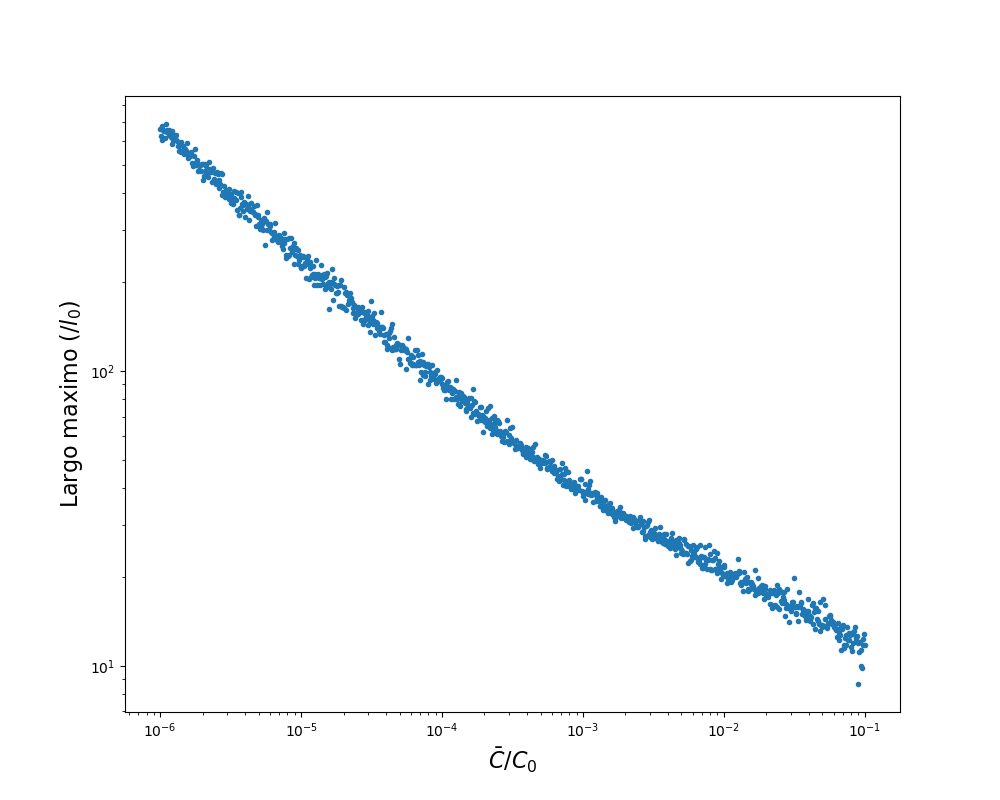
\includegraphics[width=0.8\textwidth]{graficos_inst/lmax_vs_epsilon.png}
    \caption{Largo total máximo en función de $\bar{C}/C_0$ (normalizado).}
    \label{fig:lmax_vs_epsilon}
\end{figure}

Es bastante evidente que el tamaño máximo depende de esta variable. \textbf{No es una ley de potencia??}

\section{Ley de Murray}

Uno de los objetivos es ver que la ley de Murray va a aparecer por si sola en el sistema, sin ser impuesta.
Pero esto resulta ser evidente:

Sea $C_0$ un ducto padre y $C_1$, $C_2$ sus "hijos". El ducto $C_1$ es atravesado por $Q_1$, y $C_2$ por $Q_2$, por lo que $C_0$ es atravesado
por $Q_0 = Q_1 + Q_2$. Entonces, las conductancias óptimas son:

$$ C_i^* = \frac{Q_i^{4/3} K}{S^2 l_i} \quad i\in\{0,1,2\} $$

Con $ S = \sum_{<ij>}Q_{ij}^{2/3}l_{ij} $

Luego, podemos encontrar el radio óptimo:

$$ r_i = \left( C_i^* l_i \frac{8 \mu}{\pi} \right)^{1/4} = \frac{Q_i^{1/3}}{S^{1/2}}\left(\frac{8K\mu}{\pi}\right)^{1/4}$$

Y encontramos, efectivamente:

\begin{align*}
    r_1^3 + r_2^3 & = \left(\frac{Q_1 + Q_2}{S^{3/2}}\right)\left(\frac{8K\mu}{\pi}\right)^{3/4} \\
    & = r_0^3
\end{align*}

La ley se cumple directamente!

\section{Flujos negativos}

A veces se generan $Q_{ij}$ negativos: Esto ocurre cuando el flujo debería ser 0, pero el algoritmo de pseudo-inversa
converge a un número (negativo) muy pequeño del orden de $10^{-15}$. Como además tratamos con flujos cuadrados, esto no presenta un problema.
\\
\textbf{POR HACER:}

\begin{itemize}
    \item Separar $\bar{C}$ y K
    \item Asegurarse que $C_{ij}$ estan bien escalados
\end{itemize}

\end{document}